% usar Tex Live e lualatex
% usar minted v2.9
% custom compiler argument: -shell-escape


\documentclass{../class/IFSCreport}

\usepackage[pdftex,
            pdfauthor={Prof. Jackson Lago, Dr.},
            pdftitle={},
            pdfkeywords={},
            pdfcreator={LuaLaTex, Biber},
            pdfborder={0 0 0}]{hyperref}
\usepackage{import}

\definecolor{primary}{RGB}{137, 197, 63}
\definecolor{secondary}{RGB}{234, 32, 38}

\newcommand{\plotscale}{0.51}
\newcommand{\todo}{To be done!}



%-----------------------------------------------------------------------------------------------------------------------
\date{Junho de 2024}
\author{Jackson Lago, Dr.}
\email{jackson.lago@ifsc.edu.br}
\subject{Introdução}
\title{Python}
\subtitle{Subtítulo do modelo}
\cabecalho{\textsc{Introdução ao Python} \\  \vspace{1.5mm}}

\addbibresource{refs.bib}

%-----------------------------------------------------------------------------------------------------------------------
\begin{document}

\maketitle
\tableofcontents



%\chapter{Título do capítulo}
\lipsum[1-2]

\section{Título da seção}
\lipsum[3-5]
%

\section{Equações}
Exemplo de equação:
    $$
    f(t) = \sum_{h=1,3\ldots}^\infty \dfrac{1}{h!} \sin(h \omega t)
    $$

Outro exemplo:
\begin{equation}
    \begin{bmatrix}
        d \\
        q \\
        0
    \end{bmatrix}
    =
    \frac{2}{3}
    \begin{bmatrix}
        \cos\theta & \cos(\theta - 120^\circ) & \cos(\theta + 120^\circ) \\
        \sin\theta & \sin(\theta - 120^\circ) & \sin(\theta + 120^\circ) \\
        1/2 & 1/2 & 1/2
    \end{bmatrix}
    \begin{bmatrix}
        a \\
        b \\
        c
    \end{bmatrix}
    \label{eq:abs_dq0}
\end{equation}

\begin{equation}
    \begin{bmatrix}
        d \\
        q
    \end{bmatrix}
    =
    \begin{bmatrix}
        \cos\theta & \sin\theta \\
        -\sin\theta & \cos\theta
    \end{bmatrix}
    \begin{bmatrix}
        \alpha \\
        \beta
    \end{bmatrix}
    \label{eq:parke}
\end{equation}




\section{Figuras}
\lipsum[6]

Exemplo de gráfico utilizando \texttt{tikz}:
\begin{figure}[h]
    \centering
    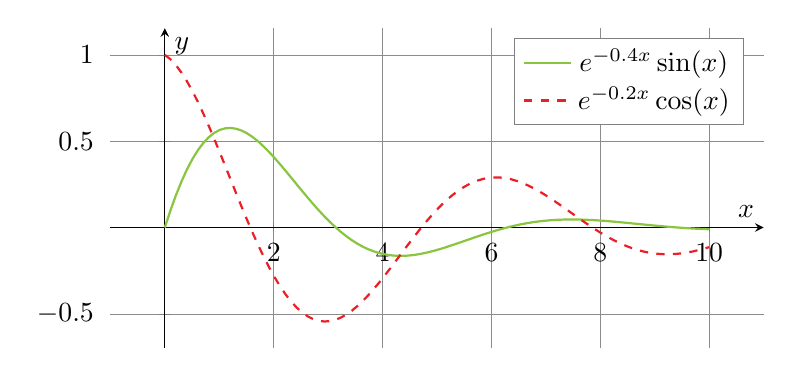
\begin{tikzpicture}
    \begin{axis}[
        width=280px,
        height=160px,
        axis lines = middle,
        enlargelimits = true,
        xlabel = $x$,
        ylabel = $y$,
        legend pos = north east,
        grid = major,
        legend style={fill=white, draw=gray, text=black},
        yticklabel style={xshift=-20pt},
        axis line style={thin},
        grid style={solid, gray!90, line width=0.2pt}
    ]
        \addplot [primary, thick, domain=0:10, samples=100]
            {exp(-0.4*x) * sin(deg(x))};
        \addlegendentry{$e^{-0.4x} \sin(x)$}

        \addplot [secondary, thick, dashed, domain=0:10, samples=100]
            {exp(-0.2*x) * cos(deg(x))};
        \addlegendentry{$e^{-0.2x} \cos(x)$}
    \end{axis}
\end{tikzpicture}
    \caption{Exemplo de figura \texttt{tikz}}
    \label{fig:exemplo}
\end{figure}


\lipsum[7]




Exemplo de imagem a partir de arquivo apresentado na \figr{fig:exemplo1}.
\begin{figure}[h]
    \centering
    
\includegraphics[width=0.3\textwidth, angle=20]{../class/figs/logo_capa}
    \caption{Exemplo de importação de figura}
    \label{fig:exemplo1}
\end{figure}

Exemplo de subfigures apresentado na \ref{fig:figuras_conjunto}, que possui as sub-figuras \ref{fig:imagem1} e \ref{fig:imagem2}.
\begin{figure}[h]
    \centering
    \begin{subfigure}{0.35\textwidth}
        \centering
        
\includegraphics[width=\linewidth, angle=90]{../class/figs/logo_capa}
        \caption{Legenda da primeira figura}
        \label{fig:imagem1}
    \end{subfigure}
    \hspace{15mm}
    \begin{subfigure}{0.35\textwidth}
        \centering
        
\includegraphics[scale=0.45, angle=45]{../class/figs/logo_capa}
        \caption{Legenda da segunda figura}
        \label{fig:imagem2}
    \end{subfigure}
    \caption{Legenda geral do conjunto de figuras}
    \label{fig:figuras_conjunto}
\end{figure}



Exemplo de imagem a partir de arquivo com anotação \texttt{tikz} apresentado na \figr{fig:exemplo2}.
\begin{figure}[h]
    \centering
    \begin{tikzpicture}
        \node[anchor=south west] (img) at (0,0) {
\includegraphics[scale=0.5]{../class/figs/logo_capa}};
        \draw[secondary, thick, line cap=round, <-] (3,1.2) -- (3.5,1.4) node[right, draw=secondary, rounded corners, thin, fill=black!85!secondary] {nota importante!};
    \end{tikzpicture}
    \caption{Exemplo de figura com anoração co. \texttt{tikz}}
    \label{fig:exemplo2}
\end{figure}



\section{Código fonte}
\lipsum[8]

Exemplo de código fonte usando ambiente \texttt{minted}:
\begin{minted}{custompython}
'''Exemplo de código definido no proprio .tex com \begin{minted}{custompython}...'''
def exemplo():
    pass
\end{minted}

\lipsum[9-11]

Exemplo de código fonte importado de arquivo usando \texttt{inputminted}:
\inputminted{custompython}{./capitulos/ex_codigo.py}
%\inputminted[linenos, firstnumber=5478]{custompython}{./capitulos/ex_codigo.py}


\section{Citações}
A referência \cite{einstein1905} é um exemplo de citação.


\unnumberedchapter{Orientações Iniciais e Convenções}

Este tutorial oferece uma introdução concisa ao Python, voltada para os alunos ingressantes no curso de Mestrado
Profissional em Sistemas de Energia.

Por ter um caráter introdutório, o texto apresenta exemplos e conceitos sem a intenção de esgotar completamente o
tema ou fornecer soluções otimizadas para problemas específicos.

Os exemplo aqui descritos assumem a utilização de Python 3.10 (ou superior) que deve estar devidamente instalado (\colorurl{https://www.python.org/downloads/}).

Também recomenda-se a utilização de alguma IDE (\emph{Integrated Development Environment}) para facilitar a escrita e manipulação do código.
As duas mais populares para desenvolvimento em Python são:
\begin{itemize}
    \item \texttt{PyCharm}: uma IDE dedicada ao Python, desenvolvida pela JetBrains.
    Oferece uma configuração padrão robusta e inclui funcionalidades como autocomplete, análise de código, refatoração,
    debugging, testes integrados e integração com Git.
    É uma ferramenta profissional ideal para projetos complexos, embora possa ser pesada em máquinas mais simples ou antigas.
    Disponível em duas versões: Professional (paga) e Community Edition (gratuita).
    Embora a versão gratuita tenha algumas limitações, ela é mais do que suficiente para este tutorial e até mesmo para projetos pessoais de grande porte.
    (\colorurl{https://www.jetbrains.com/pycharm/download/})
    \item \texttt{VS Code}: um editor de código aberto, leve e flexível, não restrito a uma única linguagem.
    O suporte ao Python é obtido por meio de extensões, que também habilitam ferramentas de análise de código.
    Seu uso exige uma configuração inicial, incluindo a instalação da extensão Python (Microsoft).
    Outras extensões relacionadas à produtividade podem ser obtidas pelo marketplace integrado ao VS Code.
    (\colorurl{https://code.visualstudio.com/download/})
\end{itemize}


No texto, códigos Python serão identificados por uma caixa preta:
\begin{minted}[escapeinside=??, frame=single, rulecolor=brown]{custompython}
?\textcolor{brown}{\faIcon{file} exemplo\_codigo\_python.py}?
\end{minted}
\vspace{-0.8em}
%
\begin{minted}[escapeinside=??]{custompython}

print('Hello, World!')
\end{minted}

enquanto comandos e mensagens impressas no terminal estarão em uma caixa azul:
\begin{minted}[escapeinside=??]{text}
?\textcolor{green!20!brown}{C:\char92curso\_python\char92>}? python exemplo_codigo_python.py
Hello, World!
\end{minted}
\chapter{Variáveis e Tipos}

A computação em seu nível mais básico baseia-se na manipulação de dados armazenados na memória.

As linguagens naturais são ambíguas e, muitas vezes, subjetivas, o que pode gerar interpretações variadas.
Diferentemente delas, uma linguagem de programação deve ser precisa e determinística, garantindo previsibilidade no
processamento da informação.

Através dessas linguagens, comunicamos ao hardware como manipular os dados armazenados na memória, transformando-os
em novos valores.
Esses valores, por sua vez, são interpretados e associados a algo significativo no mundo real, seja um número, um
texto ou uma representação visual.

Blocos de dados armazenados na memória que representam coletivamente um conceito comum são chamados objetos.
Os tipos associados a esses objetos formam uma camada de abstração que define como um conjunto de bits deve ser
interpretado.
Essa abstração permite representar diversos conceitos, como números inteiros, valores fracionários, caracteres e outros
tipos de dados, tornando a manipulação dessas informações mais estruturada e intuitiva.

Diferente de algumas linguagens, em Python não é necessário declarar o tipo da variável explicitamente
--- o interpretador determina automaticamente o tipo com base no valor atribuído.

Python possui diversos tipos primitivos, que representam os dados mais básicos da linguagem.
Estes podem ser utilizados diretamente para expressar algum conceito real ou combinados para formar tipos compostos
(ou estruturados), capazes de representar ideias e relações mais complexas.


\section{Tipos primitivos}

Os principais tipos primitivos em Python são:

\begin{itemize}
    \item \inlcode{int}: utilizado para armazenar números inteiros, como \inlcode{10}, \inlcode{-5}, e \inlcode{0}
    \item \inlcode{float}: representa valores com casas decimais, como \inlcode{3.14}, \inlcode{-0.5}, \inlcode{1.6e-3}
    \item \inlcode{complex}: representa números complexos, como \inlcode{3.2 + 4.7j}
%    \item \inlcode{bool}: representa uma grandeza booleana, que pode assumir apenas \inlcode{True} ou \inlcode{False}, essencial para estruturas de decisão
    \item \inlcode{str}: string utilizado para armazenar textos, como \inlstr{Hello, world!} ou
        \inlstrdouble{python}\footnote{Em Python, strings literais podem ser delimitadas por aspas simples
        (\inlkey{\'}) ou duplas (\inlkey{\"}). Essa flexibilidade é útil quando queremos incluir o outro tipo de aspas dentro do texto, sem a necessidade de caracteres de escape.}.
    \item \inlcode{bool}: representa uma grandeza booleana, que pode assumir apenas \inlcode{True} ou \inlcode{False}, essencial para estruturas de decisão
    \item \inlcode{NoneType}: pode assumir apenas o valor \inlcode{None}, e pode ser explicitamente atribuído
    a uma variável para sinalizar a ausência de um valor.



\end{itemize}

Em código a criação de variáveis com os tipos acima descritos ficaria:
\begin{minted}{custompython}
idade = 25
peso = 78.6
impedancia = 5 + 3j
ativo = True
nome = 'Fulano de Tal'
sem_valor = None

print(f"'idade' é uma variável do tipo {type(idade)} e valor: {idade}")
print(f"'peso' é uma variável do tipo {type(peso)} e valor: {peso}")
print(f"'impedancia' é uma variável do tipo {type(impedancia)} e valor: {impedancia}")
print(f"'ativo' é uma variável do tipo {type(ativo)} e valor: {ativo}")
print(f"'nome' é uma variável do tipo {type(nome)} e valor: {nome}")
print(f"'sem_valor' é uma variável do tipo {type(sem_valor)} e valor: {sem_valor}")
\end{minted}

O código acima apenas cria diversas variáveis de diferentes tipos e para cada uma delas imprime o seu tipo e valor no terminal:
\begin{minted}{text}
'idade' é uma variável do tipo <class 'int'> e valor: 25
'peso' é uma variável do tipo <class 'float'> e valor: 78.6
'impedancia' é uma variável do tipo <class 'complex'> e valor: (5+3j)
'ativo' é uma variável do tipo <class 'bool'> e valor: True
'nome' é uma variável do tipo <class 'str'> e valor: Fulano de Tal
'sem_valor' é uma variável do tipo <class 'NoneType'> e valor: None
\end{minted}

Antes de prosseguirmos e começarmos a utilizar essas variáveis para realizar tarefas úteis, é importante refletir
sobre o conceito de tipagem e as diferentes formas como as linguagens de programação a tratam.

Algumas linguagens possuem tipagem dinâmica, onde o tipo das variáveis é determinado durante a execução do programa.
Outras adotam tipagem estática, exigindo que os tipos sejam declarados antecipadamente e validados durante a compilação
(quando aplicável).
Essa diferença impacta diretamente a maneira como escrevemos, mantemos e depuramos código.

Python é uma linguagem interpretada e de tipagem dinâmica, o que significa que seu código não é compilado previamente
e que o tipo de uma variável é determinado em tempo de execução, sem exigir uma declaração explícita por parte do
programador.
Isso não significa que as variáveis não possuam um tipo associado, mas sim que o próprio interpretador do Python
gerencia automaticamente os tipos conforme necessário.

%Esse comportamento contrasta com linguagens de tipagem estática (como C, C++, Rust, etc.), onde a definição de tipos
%ocorre durante a compilação, antes do início da execução do programa.

Por exemplo, no seguinte código:
\begin{minted}{custompython}
descricao = 'Geladeira frost free 500l'  # tipo: str
quantidade = 10                          # tipo: int
peso_unitario = 72.7                     # tipo: float
\end{minted}

as variáveis \inlcode{descricao}, \inlcode{quantidade} e
\inlcode{peso\_unitario}\footnote{Em Python, o estilo \texttt{snake\_case} é tradicionalmente usado para nomear variáveis,
separando palavras com underscores (\texttt{\_}) e usando minúsculas.}
são automaticamente criadas com os tipos
\inlcode{str}, \inlcode{int} e \inlcode{float}, respectivamente.
O interpretador infere esses tipos com base nos valores atribuídos a cada variável
(o valor à direita de \inlcode{=}).

Além disso, uma variável pode ser redefinida posteriormente, até mesmo para um tipo diferente.
Essa abordagem pode ser vantajosa para tornar o código mais flexível e dinâmico, mas também pode introduzir problemas ao
mascarar erros difíceis de identificar.

Por exemplo, em
\begin{minted}{custompython}
descricao = 'Geladeira frost free 500l'  # tipo: str
quantidade = 10                          # tipo: int
peso_unitario = 72.7                     # tipo: float

print(f"pré: 'descricao' é do tipo {type(descricao)} com valor: {descricao}")
descricao = quantidade   # redefine descricao para int
print(f"pós: 'descricao' é do tipo {type(descricao)} com valor: {descricao}")
\end{minted}
\begin{minted}{text}
pré: 'descricao' é do tipo <class 'str'> com valor: Geladeira frost free 500l
pós: 'descricao' é do tipo <class 'int'> com valor: 10
\end{minted}

a variável \inlcode{descricao} inicialmente criada como \inlcode{str} e valor \inlstr{Geladeira frost free 500l}, é redefinida para
\inlcode{int}, passando a armazenar o valor \inlcode{10}.
Esse comportamento exemplifica a tipagem dinâmica do Python, onde uma mesma variável pode assumir diferentes tipos ao
longo da execução do código.

Em Python, uma variável é apenas um nome que referencia um objeto em memória.
Quando uma variável é redefinida, ela passa a apontar para outro objeto, que não necessariamente precisa ter o mesmo tipo.

Esse código é válido e não resultará em erros de execução por si só.
No entanto, pode representar um erro lógico caso essa alteração de tipo não esteja alinhada com a intenção do programador.
Cabe ao programador garantir a coerência do
código, tratando \inlcode{descricao} como \inlcode{str} na parte inicial do programa e como
\inlcode{int} posteriormente, conforme necessário.

Embora essa redefinição com mudança de tipo não configure um erro sintático e possa ser útil em alguns casos, sua
prática indiscriminada é desencorajada, pois pode dificultar legibilidade e a manutenção do código.

A tipagem dinâmica do Python torna a linguagem mais simples e flexível, facilitando o desenvolvimento, especialmente
para iniciantes.
No entanto, essa característica exige atenção, pois erros de tipagem podem surgir em tempo de execução se os tipos
das variáveis não forem corretamente tratados.


Por exemplo, considere o seguinte código:
\begin{minted}{custompython}
descricao = 'Geladeira frost free 500l'  # tipo: str
quantidade = 10                          # tipo: int
peso_unitario = 72.7                     # tipo: float

peso_total = peso_unitario * quantidade
print(f'Peso total: {peso_total} kg')
\end{minted}
%
\begin{minted}{text}
    Peso total: 727.0 kg
\end{minted}

As variáveis \inlcode{quantidade} (\inlcode{int}) e \inlcode{peso\_unitario} (\inlcode{float}) são multiplicadas, gerando
um novo valor do tipo \inlcode{float}, que é atribuído a \inlcode{peso\_total}.
Essa operação é perfeitamente válida, tanto do ponto de vista sintático da linguagem quanto do ponto de vista lógico.

Agora, observe o que aconteceria se o programador, por descuido, digitasse \inlcode{descricao} ao invés
de \inlcode{peso\_unitario}.
\begin{minted}{custompython}
descricao = 'Geladeira frost free 500l'  # tipo: str
quantidade = 10                          # tipo: int
peso_unitario = 72.7                     # tipo: float

peso_total = peso_unitario * descricao   # <- erro de digitação
print(f'Peso total: {peso_total} kg')
\end{minted}
%
\begin{minted}[escapeinside=??]{text}
Traceback (most recent call last):
  File ?\textcolor{magenta!80}{\char34c:\char92curso\_python\char92aula1\char92variaveis.py\char34}?, line ?\textcolor{magenta!80}{5}?, in ?\textcolor{magenta!80}{<module>}?
    peso_total = ?\textcolor{red!70}{peso\_unitario * descricao}?
                 ?\textcolor{red!70}{\char126\char126\char126\char126\char126\char126\char126\char126\char126\char126\char126\char126\char126\char126\char94\char126\char126\char126\char126\char126\char126\char126\char126\char126\char126}?
?\textcolor{magenta!80}{TypeError: can't multiply sequence by non-int of type 'float'}?
\end{minted}

Durante a execução do código, o interpretador encontrou uma operação inválida e gerou um erro de incompatibilidade
de tipos, pois a multiplicação entre um \inlcode{float} com um \inlcode{str} não está definida.

Perceba que esse erro só ocorre em tempo de execução, no momento em que o interpretador Python tenta realizar a
multiplicação entre um \inlcode{float} e um \inlcode{str}.
Trata-se de um erro de lógica, não de sintaxe, pois, sendo Python uma linguagem de tipagem dinâmica,
\inlcode{peso\_unitario} e \inlcode{descricao} poderiam armazenar qualquer tipo de dado ao longo da execução do código,
podendo sofrer mudanças não só de valor, mas também de tipo, até atingir a linha onde ocorre a tentativa e
multiplicação e, consequentemente, o erro.

Esse erro seria facilmente detectado e corrigido no momento da escrita do código ou durante a compilação em
linguagens de tipagem estática (como C, C++, Java, Rust, etc), impedindo sua ocorrência em tempo de execução.
Esse exemplo foi incluído apenas para ilustrar também as desvantágens e os possíveis desafios da tipagem dinâmica.

Embora Python não suporte tipagem estática, ele suporta opcionalmente anotação de tipos.
As anotações de tipos são declarações do programador quanto ao tipo intentado para cada variável
criada\footnote{Além da anotação de tipo de variáveis, podemos também anotar tipos para parâmetros e retorno de
funções/métodos}.

Apesar das anotações de tipos não influenciarem a execução do código --- sendo ignoradas pelo interpretador Python
durante a execução --- elas são extremamente úteis.
Essas anotações são utilizadas por ferramentas de análise estática integradas à maioria das IDEs modernas para
identificar possíveis erros de incompatibilidade de tipos no momento da escrita do
código\footnote{A análise estática de tipos (ou \emph{type checking}) está habilitada por padrão na IDE PyCham.
Já no VS Code, ela pode ser habilitada incluindo os campos
\texttt{'python.analysis.autoImportCompletions': true,} \texttt{'python.analysis.typeCheckingMode': 'standard'} no arquivo de
configurações \texttt{settings.json}.
%Outras extensões populares para produtividade como \texttt{Pylint} e \texttt{Flake8} podem ser instaladas pelo VS Code Extensions Marketplace
}
além de melhorar a legibilidade e a manutenção, minimizando assim os riscos associados à tipagem dinâmica, mantendo
todos os seus benefícios.

Reescrevendo o exemplo anterior com anotação de tipos, a IDE agora pode nos alertar sobre um provável erro antes
mesmo da execução:
\begin{minted}[escapeinside=??]{custompython}
descricao: str = 'Geladeira frost free 500l'
quantidade: int = 10
peso_unitario: float = 72.7

peso_total = peso_unitario * descricao?\tikzmark{squigglydescricao}?   # <- erro de digitação
print(f'Peso total: {peso_total} kg')
\end{minted}
%
\begin{tikzpicture}[remember picture, overlay]
    \draw[orange, thick, line cap=round, decorate, decoration={snake, amplitude=0.15mm, segment length=1.5mm}]
        (pic cs:squigglydescricao) ++(-0.01,-0.03) -- ++(-3.66,0.0);
    \draw[->, thick, line cap=round, orange] (pic cs:squigglydescricao) ++(-0.01,-0.03) -- ++(0.6,0.6) node[right, fill=black!80!orange, inner sep=1pt]
        {\scriptsize\texttt{Operator '*'~not supported for types 'float'~and 'str'}};
\end{tikzpicture}

Além dos tipo primitivos, Python possui mais duas formas de armazenar informações: através de classes customizadas
\inlcode{class}, que serão discutidas no capítulo \ref{class} e através de coleções de dados (\inlcode{collections})




\section{Collections}

Em Python, coleções são estruturas que armazenam múltiplos valores em uma única variável.
As quatro coleções mais comuns da linguagem são: \inlcode{list}, \inlcode{tuple}, \inlcode{set} e \inlcode{dict}.
Cada uma delas possui características específicas que as tornam mais adequadas para diferentes situações.



\subsection{\inlcode{list}}
As listas (\inlcode{list}) são uma das estruturas mais versáteis do Python, representam sequências de elementos
ordenados e mutáveis.
Ous seja, os elementos inseridos nela são mantidos na mesma ordem e podem ser alterados a qualquer momento,
seja adicionando, removendo modificando ou substituindo itens.

Além disso, possuem tamanho arbitrário, crescendo conforme novos elementos são inseridos.

Uma lista pode ser criada utilizando colchetes \inlcode{[]} e pode armazenar qualquer tipo de dado, inclusive, diferentes tipos para cada elemento.
Por exemplo:
\begin{minted}{custompython}
numeros = [8, 2, 0, -4, 15]                # lista de inteiros
nomes = ['Fulano', 'Beltrano', 'Sicrano']  # lista de strings
misto = [42, 'texto', 3.14, True]          # lista com tipos variados
\end{minted}

A lista é uma coleção dinâmica, e pode crescer mesmo apos sua criação para acomodar novos elementos:
\begin{minted}{custompython}
cores = ['azul', 'amarelo', 'cinza', 'vermelho']
print(f'pré: A lista 'cores' possui {len(cores)} elementos: {cores}')

cores.append('verde')  # adiciona um novo elemento de valor 'verde' ao final da lista
print(f'pós: A lista 'cores' possui {len(cores)} elementos: {cores}}')
\end{minted}
\begin{minted}{text}
pré: A lista 'cores' possui 4 elementos: ['azul', 'amarelo', 'cinza', 'vermelho']
pós: A lista 'cores' possui 5 elementos: ['azul', 'amarelo', 'cinza', 'vermelho', 'verde']
\end{minted}

Esse código introduz um elemento novo: a chamada \inlcode{cores.append()}, onde \inlcode{append()} é um método da classe
\inlcode{list}.
Métodos são semelhantes a funções, mas estão associados a um tipo de dado específico (a uma \inlcode{class}) e
normalmente modificam o próprio objeto ao qual pertencem.

A chamada de um método geralmente impacta diretamente o objeto a partir do qual ele é invocado.
No caso de \inlcode{append()}, um novo elemento é adicionado ao final da lista, alterando sua estrutura inicial.

Esse conceito será revisitado e formalizado com mais detalhes no Capítulo \ref{class}, quando exploraremos a
construção e uso de classes em Python.

Note que a lista cresce automaticamente para acomodar novos elementos, sem que o programador precise gerenciar ou
alocar memória adicional manualmente.
Essa característica torna as listas particularmente flexíveis para armazenar conjuntos dinâmicos de dados.

Além disso, no último exemplo, introduzimos a função \inlcode{len()}, que retorna o número de elementos presentes na coleção.
Essa é uma função essencial para validar o tamanho de uma lista antes de realizar operações que dependam da quantidade de itens.

Também podemos acessar elementos individuais dessa lista, tanto para leitura como para escrita.
Essa indexação é realizada com a seguinte sintaxe \inlcode{nome_da_lista[indice]}, veja o código exemplo:
\begin{minted}{custompython}
cores = ['azul', 'amarelo', 'cinza', 'vermelho', 'verde']

# a indexação dos elemntos da listas por um inteiro inicia em 0
selecionada1 = cores[1]  # indice 1 equivale ao 2° elemento
print(f'selecioanda1 é: {selecionada1}')

# indice negativos podem ser usados para indexar elemntos do final para o início da listas
selecionada2 = cores[-2]  # -2 indica o penúltimo elemento
print(f'selecioanda2 é: {selecionada2}')

# é possível a indexação por slice, ou faixa de índices m:n (n é não inclusivo)
selecionadas = cores[0:3]  # 0:3 corresponde aos indices 0,1,2
print(f'selecionadas são: {selecionadas}')

# elementos da lista também podem ser individualemente modificados
cores[2] = 'marrom'  # altera o terceiro elemento de 'cinza' para 'marrom'
print(f'pós modificação: {cores}')

# podemo excluir elementos, o que desloca dos indices dos elementos a sua direita
del cores[3]
print(f'pós excusão por indice: {cores}')

# ou ainda podemo excluir não por indice mas por valor
cores.remove('azul')
print(f'pós excusão por valor: {cores}')

# tentar acessar índices que não existe resultará em um erro
cores[99]
\end{minted}
\begin{minted}[escapeinside=??]{text}
selecioanda1 é: amarelo
selecioanda2 é: vermelho
selecionadas são: ['azul', 'amarelo', 'cinza']
pós modificação: ['azul', 'amarelo', 'marrom', 'vermelho', 'verde']
pós excusão por índice: ['azul', 'amarelo', 'marrom', 'verde']
pós excusão por valor: ['amarelo', 'marrom', 'verde']
Traceback (most recent call last):
  File ?\textcolor{magenta!80}{\char34c:\char92curso\_python\char92aula1\char92variaveis.py\char34}?, line ?\textcolor{magenta!80}{28}?, in ?\textcolor{magenta!80}{<module>}?
    ?\textcolor{red!70}{cores[99]}?
    ?\textcolor{red!70}{\char126\char126\char126\char126\char126\char94\char94\char94\char94}?
?\textcolor{magenta!80}{IndexError: list index out of range}?
\end{minted}

Vários outros métodos e funções para manipular listas estão disponíveis por padrão. Segue uma breve enumeração dos mais úteis:
\begin{itemize}
\item \inlcode{len(lista)} – Retorna o número de elementos na lista.
\item \inlcode{lista.append(valor)} – Adiciona um novo elemento ao final da lista.
\item \inlcode{lista.insert(indice, valor)} – Insere um elemento em uma posição específica.
\item \inlcode{lista.remove(valor)} – Remove a primeira ocorrência do valor especificado.
\item \inlcode{lista.pop(indice)} – Remove e retorna o elemento na posição indicada (ou o último, se omitido).
\item \inlcode{lista.index(valor)} – Retorna o índice da primeira ocorrência do valor.
\item \inlcode{lista.count(valor)} – Retorna o número de vezes que o valor aparece na lista.
\item \inlcode{lista.sort()} – Ordena a lista em ordem crescente (por padrão).
\item \inlcode{lista.reverse()} – Inverte a ordem dos elementos da lista.
\item \inlcode{sorted(lista)} – Retorna uma nova lista ordenada, sem modificar a original.
\item \inlcode{lista.copy()} – Retorna uma cópia superficial da lista.
\item \inlcode{lista.clear()} – Remove todos os elementos da lista.
\end{itemize}

Esses métodos permitem desde operações simples, como acessar elementos, até manipulações mais avançadas,
como ordenação e remoção de elementos.
No decorrer desse tutorial, abordaremos mais detalhes sobre a aplicação desses métodos em exemplos práticos.


\subsection{\inlcode{tuple}}

Assim como \inlcode{list}, a \inlcode{tuple} (ou tupla) é uma estrutura de dados que permite armazenar uma sequência
de valores.
No entanto, enquanto listas são mutáveis (ou seja, seus elementos podem ser alterados, adicionados ou removidos),
tuplas são imutáveis: uma vez criadas, seus elementos não podem ser modificados.

Essa característica confere à tupla maior segurança e previsibilidade, tornando-a ideal para representar coleções
fixas de dados que não devem ser alteradas acidentalmente, ou até valores de retorno de uma função.

Tuplas são definidas por uma sequência de valores separados por vírgula (\inlcode{,}), não necessariamente, mas comumente
inseridos entre parênteses (\inlcode{()}).
\begin{minted}{custompython}
coordenada = (46.8, 22.3)
print(coordenada)
\end{minted}
\begin{minted}[escapeinside=??]{text}
(46.8, 22.3)
\end{minted}

Para definir uma tupla de um único elemento, é obrigatório adicionar uma vírgula,
caso contrário, o Python interpretará o valor como um tipo isolado:
\begin{minted}{custompython}
numero = (5)   # não é tupla, é apenas um int
tupla = (5,)  # tupla com um único elemento
print(f'numero é do tipo {type(numero)} e valor: {numero}')
print(f'tupla é do tipo {type(tupla)} e valor: {tupla}')
\end{minted}
\begin{minted}[escapeinside=??]{text}
numero é do tipo <class 'int'> e valor: 5
tupla é do tipo <class 'tuple'> e valor: (5,)
\end{minted}


A indexação de tuplas segue o mesmo princípio das listas,
permitindo acessar elementos por índices (\inlcode{0} para o primeiro item, índices negativos para contar do final)
\begin{minted}{custompython}
cores = 'azul', 'verde', 'vermelho', 'amarelo', 'roxo'
print(cores[0])     # azul
print(cores[-1])    # roxo
print(cores[1:4])   # ('verde', 'vermelho', 'amarelo')
\end{minted}
\begin{minted}[escapeinside=??]{text}
azul
roxo
('verde', 'vermelho', 'amarelo')
\end{minted}

Embora tupla possa parecer uma versão limitada de lista, elas são estruturas complementares, com propósitos distintos.
Essas limitações justamente tornam operações com tuplas mais previsíveis, rápidas e seguras.




\subsection{\inlcode{set}}
Um \inlcode{set} é uma coleção semelhante à lista (\inlcode{list}), porém não permite valores duplicados e não mantém uma ordem fixa dos
elementos.
Isso faz com que seja uma estrutura útil para armazenar itens únicos e realizar operações como união,
interseção e diferença.

Os conjuntos podem ser criados utilizando chaves \inlcode{\{\}} ou a função \inlcode{set()}:
\begin{minted}{custompython}
cores = {'azul', 'vermelho', 'verde', 'azul'}
print(cores)
\end{minted}
\begin{minted}[escapeinside=??]{text}
{'azul', 'vermelho', 'verde'}
\end{minted}

Observe que, mesmo que \inlstr{azul} tenha sido declarado duas vezes, ele aparece apenas uma vez no conjunto.

Outra forma de criar um conjunto é utilizando \inlcode{set()} passando uma \inlcode{list} como argumento:
\begin{minted}{custompython}
valores = set([1, 2, 3, 4, 4, 5])
print(valores)
\end{minted}
\begin{minted}[escapeinside=??]{text}
{1, 2, 3, 4, 5}
\end{minted}

Os conjuntos são ideais quando precisamos garantir que os elementos sejam únicos, eliminando valores repetidos automaticamente.

Por não manter uma ordem fixa dos elementos, \inlcode{set} não permite acesso por índice.
Isso significa que não podemos utilizar a notação \inlcode{set[indice]} para recuperar ou modificar elementos
específicos, como fazemos com listas.
Em vez disso, a manipulação de conjuntos é realizada por métodos próprios, como adição, remoção, união, interseção e
diferença, que operam sobre o conjunto como um todo:

\begin{minted}{custompython}
a = {1, 2, 3, 4}
b = {3, 4, 5}
b.add(6)

print(f'união: {a | b}')
print(f'interseção: {a & b}')
print(f'diferença: {a - b}')
\end{minted}
\begin{minted}[escapeinside=??]{text}
união: {1, 2, 3, 4, 5, 6}
interseção: {3, 4}
diferença: {1, 2}
\end{minted}

Embora \inlcode{set} não suporte indexação direta, ainda é possível iterar sobre seus elementos utilizando laços
como \inlcode{for}.
Dessa forma, podemos percorrer todos os itens do conjunto sem precisar acessar um elemento
específico por índice.
A iteração sobre coleções de dados será abordada no capítulo \ref{iffor}.

Aqui está uma lista resumida dos principais métodos e funções para manipulação de \inlcode{set} em Python:
\begin{itemize}
\item \inlcode{len(set)} – Retorna o número de elementos no conjunto.
\item \inlcode{set.add(valor)} – Adiciona um novo elemento ao conjunto.
\item \inlcode{set.remove(valor)} – Remove um elemento existente (gera erro se o valor não existir).
\item \inlcode{set.discard(valor)} – Remove um elemento sem gerar erro caso ele não exista.
\item \inlcode{set.pop()} – Remove e retorna um elemento aleatório do conjunto.
\item \inlcode{set.clear()} – Remove todos os elementos do conjunto.
\item \inlcode{set.copy()} – Retorna uma cópia do conjunto.
\end{itemize}


\subsection{\inlcode{dict}}

Em Python, um dicionário (\inlcode{dict}) é uma estrutura de dados que implementa uma \emph{hash table}, permitindo o armazenamento de pares
\inlcode{key: value} (chave e valor).
Essa abordagem garante acesso eficiente aos valores a partir de suas chaves, tornando a busca em grandes coleções
extremamente rápida.

Diferente das listas (\inlcode{list}) e conjuntos (\inlcode{set}), que organizam elementos sequencialmente ou de forma desordenada,
o dicionário associa cada valor a uma chave única, permitindo acessos diretos sem necessidade de percorrer toda a
estrutura. Ná prática, essas chaves funcionam como os índices em listas.

Cada chave (\inlcode{key}) pode ser qualquer tipo de dado que suporte a função \inlcode{hash()}, como números, strings
ou tuplas imutáveis.
Já o valor (\inlcode{value}) pode ser qualquer objeto do Python, incluindo listas, outras coleções, classes definidas
pelo usuário e até mesmo funções.

Podemos criar um dicionário utilizando chaves (\inlcode{\{\}}) e inserindo os pares \inlcode{key: value} dentro delas.
Por exemplo:
\begin{minted}{custompython}
dados = {'nome': 'Fulano', 'idade': 25, 'cidade': 'Florianópolis'}
print(dados)
\end{minted}
\begin{minted}[escapeinside=??]{text}
{'nome': 'Fulano', 'idade': 25, 'cidade': 'Florianópolis'}
\end{minted}

Para recuperar um valor armazenado em um dicionário, utilizamos sua chave entre colchetes \inlcode{[]}:
\begin{minted}{custompython}
dados = {'nome': 'Fulano', 'idade': 25, 'cidade': 'Florianópolis'}
nome = dados['nome']
print(f'nome: {nome}')
\end{minted}
\begin{minted}[escapeinside=??]{text}
nome: Fulano
\end{minted}

Tentar acessar uma chave inexistente gera um erro \inlcode{KeyError}:
\begin{minted}{custompython}
dados = {'nome': 'Fulano', 'idade': 25, 'cidade': 'Florianópolis'}
telefone = dados['telefone']
\end{minted}
\begin{minted}[escapeinside=??]{text}
Traceback (most recent call last):
  File ?\textcolor{magenta!80}{\char34c:\char92curso\_python\char92aula1\char92variaveis.py\char34}?, line ?\textcolor{magenta!80}{2}?, in ?\textcolor{magenta!80}{<module>}?
    ?\textcolor{red!70}{telefone = dados['telefone']}?
    ?\textcolor{red!70}{           \char126\char126\char126\char126\char126\char94\char94\char94\char94\char94\char94\char94\char94\char94\char94\char94\char94}?
?\textcolor{magenta!80}{KeyError: 'telefone'}?
\end{minted}

Já escrever em uma chave previamente inexistes, expande o \inlcode{dict} incluindo esse novo par:
\begin{minted}{custompython}
dados = {'nome': 'Fulano', 'idade': 25, 'cidade': 'Florianópolis'}

dados['telefone'] = '(48)99999-9999'
print(dados)
\end{minted}
\begin{minted}[escapeinside=??]{text}
{'nome': 'Fulano', 'idade': 25, 'cidade': 'Florianópolis', 'telefone': '(48)99999-9999'}
\end{minted}

Dicionários são mutáveis, permitindo que seus elementos sejam alterados, adicionados ou removidos.
Podemos modificar ou remover um valor acessando sua chave diretamente:
\begin{minted}{custompython}
dados = {'nome': 'Fulano', 'idade': 25, 'cidade': 'Florianópolis'}

dados['idade'] = 26   # modifica o valor associado à chave 'idade'
del dados['cidade']   # remove o valor associado à chave 'cidade'
print(dados)
\end{minted}
\begin{minted}[escapeinside=??]{text}
{'nome': 'Fulano', 'idade': 26}
\end{minted}


Aqui estão alguns métodos úteis para trabalhar com dicionários:
\begin{itemize}
\item \inlcode{len(dicionario)}: Retorna a quantidade de pares chave-valor no dicionário.
\item \inlcode{dicionario.keys()}: Retorna todas as chaves do dicionário.
\item \inlcode{dicionario.values()}: Retorna todos os valores do dicionário.
\item \inlcode{dicionario.items()}: Retorna todos os pares chave-valor como tuplas.
\item \inlcode{dicionario.pop(chave)}: Remove um item e retorna seu valor.
\item \inlcode{dicionario.update(outro_dicionario)}: Atualiza o dicionário com novos pares chave-valor.
\item \inlcode{dicionario.clear()}: Remove todos os elementos do dicionário.
\end{itemize}

Dicionários são ferramentas poderosas para armazenar e acessar dados de forma eficiente.
Eles são amplamente utilizados em Python para estruturar informações e otimizar operações de busca.





\section{Referência e mutabilidade na atribuição de variáveis}

Em Python, as variáveis não armazenam diretamente os valores, mas referências para objetos na memória.
Dessa forma, o efeito da atribuição (\inlcode{=}) a uma variável depende da mutabilidade do objeto que ela
referencia, definindo se a variável continuará apontando para o mesmo objeto ou passará a referenciar um novo.

Os objetos em Python são divididos em dois grupos: imutáveis e mutáveis, conforme sua capacidade de sofrer alterações
após a criação.

Objetos imutáveis, como \inlcode{int}, \inlcode{float}, \inlcode{str}, \inlcode{bool} e \inlcode{tuple}, não podem ser
modificados após sua criação.
Qualquer operação que tente alterar uma variável que referencia um imutável resulta na criação de um novo objeto,
com um novo endereço de memória, e a variável passa a apontar para ele, sem afetar o objeto original.


Por outro lado, objetos mutáveis, como \inlcode{list}, \inlcode{dict}, \inlcode{set} e instâncias de classes, permitem
alterações diretas em seu conteúdo sem a necessidade de criar um novo objeto.
Assim, modificações feitas em uma referência são refletidas em todas as variáveis que apontam para o mesmo objeto.

Veja um exemplo com variáveis imutáveis, como \inlcode{int}:
\begin{minted}{custompython}
x = 10    # x referencia um inteiro imutável
print(f"{type(x)=}, {id(x)=}, {x}")

y = x    # y agora referencia o mesmo objeto que x
print(f"{type(y)=}, {id(y)=}, {y}")

y = y + 5    # um novo objeto é criado e y passa a referenciá-lo
print(f"{type(y)=}, {id(y)=}, {y}")

z = 10    # uma nova variável z referencia o inteiro 10
print(f"{type(z)=}, {id(z)=}, {z}")
\end{minted}
\begin{minted}{text}
type(x)=<class 'int'>, id(x)=140706534401224, 10
type(y)=<class 'int'>, id(y)=140706534401224, 10
type(y)=<class 'int'>, id(y)=140706534401384, 15
type(z)=<class 'int'>, id(z)=140706534401224, 10
\end{minted}

A função \inlcode{id(x)}, utilizada em \inlcode{print}, retorna o identificador único do objeto referenciado
por \inlcode{x}, que equivale ao seu endereço de memória na implementação CPython.

A saída do código mostra que \inlcode{x} e \inlcode{y} inicialmente referenciam o mesmo objeto \inlcode{10},
compartilhando o mesmo identificador único (\inlcode{id}). No entanto, ao modificar \inlcode{y}, Python cria um novo
objeto com valor \inlcode{15}, e \inlcode{y} passa a apontar para ele, sem alterar \inlcode{x}.


Já \inlcode{z}, criado posteriormente, também referencia o objeto \inlcode{10}.
Como esse valor é um inteiro imutável, Python pode reutilizar a mesma referência na
memória\footnote{Essa reutilização de objetos é uma otimização da implementação CPython conhecida como
\emph{internin}, geramente aplicada para pequenos objetos.}, garantindo que o
objeto permaneça inalterável.
Dessa forma, qualquer modificação em \inlcode{x} faz com que ele passe a apontar para outro objeto, sem
impactar \inlcode{z}.


Agora, um exemplo similar com variáveis mutáveis (lista de um elemento inteiro):
\begin{minted}{custompython}
x = [10]    # x referencia um lista mutável com apenas um elemento
print(f"{type(x)=}, {id(x)=}, {x}")

y = x    # y agora referencia o mesmo objeto que x
print(f"{type(y)=}, {id(y)=}, {y}")

y[0] = y[0] + 5    # nenhum novo objeto é criado, o valor em y[0] é alterado
print(f"{type(y)=}, {id(y)=}, {y}")

z = [10]    # uma nova variável z, idêntica, mas independente de x
print(f"{type(z)=}, {id(z)=}, {z}")
\end{minted}
\begin{minted}{text}
type(x)=<class 'list'>, id(x)=1945482649600, [10]
type(y)=<class 'list'>, id(y)=1945482649600, [10]
type(y)=<class 'list'>, id(y)=1945482649600, [15]
type(z)=<class 'list'>, id(z)=1945484459648, [10]
\end{minted}

Neste caso, \inlcode{x} e \inlcode{y} são referências para a mesma lista, que é mutável.
Ao modificar \inlcode{y[0]}, o conteúdo da lista é alterado diretamente, sem criar um novo objeto, o que é evidenciado
pelo fato de que o identificador único (\inlcode{id}) permanece o mesmo.

Já \inlcode{z} contém outra lista \inlcode{[10]}, alocada em um novo espaço de memória, o que explica seu
identificador diferente.

Caso se deseje copiar os valores de uma lista para outra, em vez de apenas referenciar o mesmo objeto,
é necessário usar \inlcode{copy()} ou \inlcode{deepcopy()}.

A função \inlcode{copy()} cria uma nova lista contendo os mesmos elementos da lista original, mas se algum elemento
for um objeto mutável, como outra lista ou um dicionário, a cópia conterá apenas referências para esses objetos, e
modificações nos elementos internos afetarão ambas as listas.

Já \inlcode{deepcopy()} copia recursivamente todos os objetos mutáveis dentro da estrutura, garantindo que cada
nível da cópia seja independente da original.

Veja o exemplo:
\begin{minted}{custompython}
from copy import deepcopy

x = [10]    # lista mutável com apenas um elemento
print(f"{type(x)=}, {id(x)=}, {x}")

y = x    # y agora referencia o mesmo objeto que x
print(f"{type(y)=}, {id(y)=}, {y}")

z = deepcopy(x)    # nova lista com copias dos valores de x
print(f"{type(z)=}, {id(z)=}, {z}")
\end{minted}
\begin{minted}{text}
type(x)=<class 'list'>, id(x)=2511057429440, [10]
type(y)=<class 'list'>, id(y)=2511057429440, [10]
type(z)=<class 'list'>, id(z)=2511059612160, [10]
\end{minted}

A compreensão da mutabilidade será crucial quando analisarmos a passagem de argumentos para funções,
tema abordado no próximo capítulo.






























\chapter{Expressões e Funções}

Uma expressão é qualquer fragmento de código que, ao ser executado, retorna um valor.
Ela pode ser composta por valores, variáveis, operadores e chamadas de funções, que são avaliadas para produzir um
resultado.
Esse resultado pode ser armazenado em uma variável ou utilizado como entrada para outra expressão ou função.



Um exemplo comum de expressão são as operações aritméticas:
\begin{minted}{custompython}
a = 3
b = 7

y = a * 5 + b
\end{minted}

Aqui, as variáveis \inlcode{a} e \inlcode{b} são inicializadas com valores fixos (ou \emph{literals}, como são
chamados em programação), enquanto \inlcode{y}
recebe o resultado do processamento da expressão \inlcode{a * 5 + b}, que retorna \inlcode{22}.

Os operadores aritméticos em Python são:
adição (\inlcode{+}),
subtração (\inlcode{-}),
multiplicação (\inlcode{*}),
divisão (\inlcode{/}),
divisão inteira (\inlcode{//}),
resto da divisão (\inlcode{\%}) e
potenciação (\inlcode{**}).



\section{Funções}

Outro pilar essencial da programação são as funções, que permitem a organização e reutilização de código.
Elas ajudam a evitar repetições desnecessárias, encapsular blocos lógicos e contribuir para uma estrutura mais
eficiente e modular.

Uma função é um bloco de código reutilizável, projetado para executar uma ação específica.
Sua declaração possui três elementos fundamentais:
\begin{enumerate}
\item Parâmetros de entrada, que atuam como espaços reservados para valores que serão fornecidos posteriormente
\item quando a função for chamada.
\item O corpo da função, onde a lógica é definida e executada.
\item O valor de retorno, que é o resultado da função após seu processamento.
\end{enumerate}

Quando chamamos a função, fornecemos argumentos, que são os valores reais atribuídos aos parâmetros de entrada.
Esses argumentos carregam informações essenciais vindas do contexto externo, ou seja, da parte do programa que chamou
a função.
A função, então, processa esses dados e executa a lógica necessária para produzir um resultado.

Outro aspecto crucial das funções é o escopo de suas variáveis locais (internas).
Variáveis criadas dentro de uma função existem apenas durante sua execução e são automaticamente descartadas ao seu
término.
Isso evita interferências indesejadas em outras partes do código e melhora a eficiência do uso de memória.

Para ilustrar esse conceito, podemos criar a função \inlcode{eq\_reduzida\_reta()}, que encapsula o processamento da
expressão matemática utilizada anteriormente.
Nesse caso, ela receberá três parâmetros de entrada: \inlcode{a}, \inlcode{b} e \inlcode{x}.
No corpo da função, a expressão matemática será avaliada para calcular \inlcode{y},
que será então retornado como resultado.

A chamada a essa função constitui uma expressão, de forma que esse valor de retorno pode ser capturado e armazenado
em uma variável ou usada como valor para outra expressão, ou ainda como argumento para outra função.

Veja como essa função pode ser definida em Python:
\begin{minted}{custompython}
# definição da função
# não executa nenhum código, apenas define o que será executado quando a função for chamada
def eq_reduzida_reta(a, x, b):
    y = a * x + b
    return y

# chamada da função com diferentes argumentos
resultado1 = eq_reduzida_reta(3, 5, 7)  # argumentos posicionais 3, 5, 7
resultado2 = 5 + eq_reduzida_reta(4, 2, 6)  # resultado como entrada para uma expressao
resultado3 = eq_reduzida_reta(x=-2, b=10, a=2)  # argumentos nomeados

print(f'resultado1: {resultado1}')
print(f'resultado2: {resultado2}')
print(f'resultado3: {resultado3}')
\end{minted}
\begin{minted}{text}
resultado1: 22
resultado2: 19
resultado3: 6
\end{minted}

A declaração da função é indicada pela \emph{keyword} \inlcode{def}, seguida do nome da função e pela lista de
parâmetros de entrada, declarados entre parênteses.
Após os dois pontos (\inlcode{:}), inicia-se o corpo da função.


Diferente de algumas outras linguagens onde a indentação é apenas estética, em Python ela é essencial, pois define
o bloco de código pertencente à função.
Isso garante a organização da estrutura e evita ambiguidades na execução.

Por fim, o comando \inlcode{return} especifica o valor que será retornado ao invocador da função.
Se omitida, a função não retorna um valor explícito, e seu retorno será implicitamente \inlcode{None}.

Uma chamada de função é feita pelo seu nome, seguido por um par de parênteses.
Dentro dos parênteses, passamos os argumentos, que devem corresponder aos parâmetros definidos pela função.

Em Python, essa correspondência pode ocorrer de duas formas:
\begin{itemize}
\item Argumentos posicionais, em que os valores são passados na ordem definida pela função.
\item Argumentos nomeados, onde especificamos explicitamente qual valor será atribuído a cada parâmetro,
permitindo uma ordem arbitrária.
\end{itemize}

Também podemos combinar ambos os tipos de argumentos em uma chamada de função.
No entanto, os argumentos posicionais devem obrigatoriamente vir primeiro, seguidos pelos nomeados.

Python também permite a definição de parâmetros opcionais, o que proporciona maior flexibilidade na chamada de funções.
Isso significa que ao invocar uma função, podemos fornecer todos os argumentos necessários, ou omitir aqueles marcados
como opcionais.

Um parâmetro é considerado opcional quando, na definição da função, atribuímos a ele um valor padrão.
Esse valor será usado automaticamente caso o chamador da função não forneça um argumento correspondente.

Por exemplo, podemos reescrever a função \inlcode{eq_reduzida_reta()} tornando \inlcode{b} um parâmetro opcional,
atribuindo a ele um valor padrão de \inlcode{0}.
O código correspondente seria:
\begin{minted}{custompython}
# definição da função com parâmetro opcional
def eq_reduzida_reta(a, x, b=0):
    y = a * x + b
    return y

# chamada da função com diferentes quantidades de argumentos
resultado1 = eq_reduzida_reta(3, 5, 7)  # arg b = 7 (fornecido explicitamente)
resultado2 = eq_reduzida_reta(3, 5)     # arg b omitido, valor padrão é usado (b=0)

print(f'resultado1: {resultado1}')
print(f'resultado2: {resultado2}')
\end{minted}
\begin{minted}{text}
resultado1: 22
resultado2: 15
\end{minted}

Esse conceito permite maior flexibilidade na chamada de funções, reduzindo a necessidade de fornecer todos os
argumentos manualmente quando faz sentido na lógica da função possuir comportamento padrão.
Se não indicarmos um valor para \inlcode{b}, a função usará automaticamente \inlcode{b=0}.
Os demais parâmetros (\inlcode{a} e \inlcode{b}) não possuem valor padrão, portanto, são obrigatórios.
Chamar a função sem fornecê-los resultaria em um erro.


Assim como na criação de variáveis, também podemos anotar os tipos dos parâmetros e do valor de retorno de uma função.
Essas anotações não afetam a execução do programa, pois são ignoradas pelo interpretador durante a execução.
No entanto, elas podem ser analisadas por um \emph{type checker} da IDE, que alerta sobre possíveis incompatibilidades
antes da execução do código.

Isso melhora a legibilidade do código e ajuda na detecção de erros potenciais, tornando a programação mais segura e
organizada, além de documentar as intenções do programador quando escreveu tal função.
\begin{minted}[escapeinside=??]{custompython}
# definição da função com parâmetro opcional e anotação te tipos esperados
def eq_reduzida_reta(a: int, x: int, b: int = 0) -> int:
    y = a * x + b
    return y

# chamada da função
resultado1 = eq_reduzida_reta(3, 5.6?\tikzmark{squiggly2}?, 7)    # 'float' incompatível com declaração
resultado2 = eq_reduzida_reta(3, 'texto'?\tikzmark{squiggly}?)   # 'str' incompatível com declaração
resultado3 = eq_reduzida_reta(3, 5, 7)      # ok
\end{minted}
\begin{tikzpicture}[remember picture, overlay]
    \draw[orange, thick, line cap=round, decorate, decoration={snake, amplitude=0.15mm, segment length=1.5mm}]
        (pic cs:squiggly) ++(-0.01,-0.03) -- ++(-1.0,0.0);
    \draw[->, thick, line cap=round, orange] (pic cs:squiggly) ++(-0.01,-0.03) -- ++(0.9,0.9) node[right, fill=black!80!orange, inner sep=1pt]
        {\scriptsize\texttt{'Literal['texto']'~is not assignable to 'int'}};
    %
    \draw[orange, thick, line cap=round, decorate, decoration={snake, amplitude=0.15mm, segment length=1.5mm}]
        (pic cs:squiggly2) ++(-0.01,-0.03) -- ++(-0.4,0.0);
    \draw[->, thick, line cap=round, orange] (pic cs:squiggly2) ++(-0.01,-0.03) -- ++(0.9,0.9) node[right, fill=black!80!orange, inner sep=1pt]
        {\scriptsize\texttt{'float'~is not assignable to 'int'}};
\end{tikzpicture}

Aqui, todos os parâmetros de entrada e o valor de retorno foram definidos com o tipo \inlcode{int}, o que garante que
apenas números inteiros sejam aceitos.
Se um valor \inlcode{str} ou \inlcode{float} for passado incorretamente, um \textit{type checker} pode alertar sobre a
incompatibilidade.

Contudo, para essa função em específico, números fracionários (\inlcode{float}) seriam completamente válidos.
Para permitir esse tipo de entrada, podemos utilizar anotações de múltiplos tipos com o operador \inlcode{|}, como no
exemplo abaixo:
\begin{minted}{custompython}
# Definição da função com suporte a múltiplos tipo
def eq_reduzida_reta(a: int | float, x: int | float, b: int | float = 0) -> int | float:
    y = a * x + b
    return y
\end{minted}

Além disso, nada impede que parâmetros e valores de retorno tenham tipos diferentes—tudo depende da lógica que a
função deve executar.
A anotação de tipos é opcional, mas é altamente encorajada para manter a clareza do código e detectar possíveis erros
antes da execução.

Inda sobre funções, os parâmetros de entrada e o valor de retorno são elementos opcionais em uma função e sua presença
depende da ação que se deseja realizar.
Algumas funções podem simplesmente executar uma tarefa sem receber valores externos ou sem produzir e retornar um
resultado.

Um exemplo disso é a função padrão \inlcode{print}, que já utilizamos ao longo deste material sem muitas explicações.
Essa função recebe um argumento, geralmente uma \inlcode{str} contendo o texto a ser exibido, e imprime essa informação
no terminal.
No entanto, ela não retorna um valor\footnote{Tecnicamente, toda função python tem um retorno. Se \inlcode{retorn} não for usado dentro da função então por padrão o interpretador Python retornará \inlcode{None}, que justamente é o objeto que indica a ausência de valor.} para quem a chamou no código.

Internamente ela apenas faz uma chamada para o sistema operacional para imprimir um texto no terminal.

Em Python, funções também podem retornar múltiplos valores simultaneamente, o que torna o código mais flexível e evita
a necessidade de usar estruturas, listas ou dicionários para armazenar múltiplos resultados.

Essa funcionalidade é especialmente útil quando uma função precisa retornar vários cálculos ou informações
relacionadas ao mesmo tempo, além de possibilitar o retorno de dados sobre erros encontrados durante sua execução

Isso é possível porque Python permite que uma função retorne uma \inlcode{tupla}, que pode ser desempacotada na chamada
da função.
Veja um exemplo:
\begin{minted}{custompython}
import math

def bhaskara(a: float, b: float, c: float) -> tuple[float, float]:
    delta = b**2 - 4*a*c
    if delta < 0:
        raise ValueError("A equação não possui raízes reais. O delta é negativo.")

    raiz1 = (-b + math.sqrt(delta)) / (2 * a)
    raiz2 = (-b - math.sqrt(delta)) / (2 * a)
    return raiz1, raiz2    # retorna ambas as raízes

r1, r2 = bhaskara(a=0.5, b=14.3, c=45.0)
print(f'{r1 = }')
print(f'{r2 = }')
\end{minted}
\begin{minted}{text}
r1 = -3.5999999999999996
r2 = -25.0
\end{minted}

Observe que \inlcode{return} retorna uma \inlcode{tuple} contendo dois valores do tipo \inlcode{float}.
Essa tupla é então desempacotada pelo código que chama a função, e cada valor retornado é atribuído a uma
variável distinta (\inlcode{r1} e \inlcode{r2}).

No código acima, a linha \inlcode{import math} é uma declaração ao interpretador para importar o módulo \inlcode{math},
já que \inlcode{sqrt}, usada para calcular a raiz quadrada, não é uma função embutida (não está disponível por padrão).
No entanto, ela faz parte da biblioteca padrão do Python, então não é necessário instalar nenhum pacote externo de terceiros.

Ainda nesse exemplo, introduzimos o comando \inlcode{raise}, que lança uma exceção (geralmente associada a um erro)
caso a função encontre raízes complexas, uma condição para a qual ela não foi projetada para lidar.
Se essa exceção não for tratada\footnote{O tratamento adequado de exceções em Python é realizado por meio da estrutura \inlcode{try-except}, permitindo capturar
e gerenciar erros de maneira controlada.
No entanto, essa abordagem foge ao escopo desse texto introdutório.} pelo código que chama a função, a execução do programa será interrompida.



\section{Mutabilidade dos argumentos de funções}

Outro aspecto importante sobre funções em Python é que os argumentos são sempre passados por referência (compartilhamento de objeto).
Ou seja, os nomes das variáveis dentro da função apontam para os mesmos objetos que foram passados como argumento.

No entanto, há uma diferença de comportamento entre objetos imutáveis
(como \inlcode{int}, \inlcode{float}, \inlcode{str}, \inlcode{bool} e \inlcode{tuple}) e objetos mutáveis
(como \inlcode{list}, \inlcode{dict}, \inlcode{set} e classes definidas pelo usuário):


\begin{itemize}
\item Objetos imutáveis não podem ser alterados diretamente.
Por isso, mesmo que a referência seja compartilhada, qualquer tentativa de modificação resulta na criação de um novo objeto.
Na prática, eles se comportam como se fossem passados por cópia.

\item Já objetos mutáveis podem ser alterados diretamente.
Isso significa que modificações feitas dentro da função afetam o objeto original fora dela.

\end{itemize}

Abaixo vemos um exemplo de uma função que recebe uma variável imutável:
\begin{minted}{custompython}
def quadrado(x):
    print(f"dentro da função antes da modificação: {id(x)=}, {x=}")
    x = x**2
    print(f"dentro da função após a modificação: {id(x)=}, {x=}")

a = 5
quadrado(a)
print(f"fora da função: {id(a)=}, {a=}")
\end{minted}
\begin{minted}{text}
dentro da função antes da modificação: id(x)=140706763580456, x=5
dentro da função após a modificação: id(x)=140706763581096, x=25
fora da função: id(a)=140706763580456, a=5
\end{minted}

Fica evidente que a instrução \inlcode{x = x**2} não modifica o objeto originalmente apontado por \inlcode{x}, mas sim
cria um novo objeto em uma nova posição da memória. A variável \inlcode{x} passa, então, a referenciar esse novo objeto,
ocultando (ou \emph{shadowing}) a referência anterior dentro do escopo da função. A variável \inlcode{a}, fora da função,
permanece inalterada, continuando a referenciar o objeto original.

Agora, observe o comportamento distinto ao lidarmos com argumentos mutáveis:
\begin{minted}{custompython}
def quadrado(x):
    print(f"dentro da função antes da modificação: {id(x)=}, {x=}")
    x[0] = x[0]**2
    x[1] = x[1]**2
    print(f"dentro da função após a modificação: {id(x)=}, {x=}")

a = [5, 3]
quadrado(a)
print(f"fora da função: {id(a)=}), {a=}")
\end{minted}
\begin{minted}{text}
dentro da função antes da modificação: id(x)=2075912921088, x=[5, 3]
dentro da função após a modificação: id(x)=2075912921088, x=[25, 9]
fora da função: id(a)=2075912921088), a=[25, 9]
\end{minted}

Como a lista é um objeto mutável, a função altera diretamente o conteúdo do objeto referenciado,
mantendo o mesmo \inlcode{id}.
Isso mostra como mudanças feitas dentro da função refletem fora dela --- o parâmetro ainda aponta para o mesmo objeto,
agora modificado.


Compreender essa distinção é fundamental, pois muitas funções em Python podem não retornar um valor explícito, mas
ainda assim modificar o estado de objetos mutáveis passados como argumento.
Esse comportamento pode gerar efeitos colaterais significativos na execução do programa --- especialmente quando
não é antecipado pelo desenvolvedor.


Por outro lado, esse mecanismo também é uma ferramenta poderosa para evitar cópias desnecessárias de objetos grandes,
permitindo que funções operem diretamente sobre estruturas complexas sem comprometer o desempenho ou o uso de memória.


Funções desse tipo --- que alteram diretamente os dados aos quais têm acesso --- são conhecidas como funções com
efeitos colaterais (\emph{side-effect functions}) e são bastante comuns em operações sobre estruturas de dados,
como listas, dicionários ou objetos de classes definidas pelo usuário.

O oposto de uma \emph{side-effect function} é uma função pura (\emph{pure function}).
Funções puras garantem que seus parâmetros de entrada sejam apenas lidos, sem qualquer modificação.
Isso é possível mesmo quando se trabalha com objetos mutáveis, desde que se evite alterar seu estado.
Para isso, é comum criar cópias dos objetos antes de aplicar transformações --- o que preserva a integridade dos
dados originais, mas implica em custos de duplicação do objeto, com maior uso de memória e tempo de processamento.

Em Python, a cópia de objetos pode ser realizada com as funções \inlcode{copy()} ou \inlcode{deepcopy()} do módulo
\inlcode{copy}, dependendo da profundidade desejada.



\section{Recursão}

Outro aspecto importante das funções é que elas permitem a implementação de algoritmos ou soluções com estrutura
recursiva --- ou seja, funções que chamam a si mesmas durante a execução.

Essa abordagem pode ser útil quando um problema pode ser naturalmente decomposto em subtarefas menores de mesma
natureza.
Entre os exemplos mais comuns estão a exploração de estruturas hierárquicas, geração de combinações, percurso de
árvores binárias, execução de buscas binárias, dentre outros.
Diversos algoritmos de cálculo numérico também fazem uso de estratégias recursivas, como o método da bisseção para
encontrar raízes de funções, algoritmos de ordenação como o merge sort e a transformada rápida de Fourier (FFT).

Um exemplo clássico é a implementação de uma função que calcula o fatorial de um número, já que $n! = n \cdot (n-1)!$:
\begin{minted}{custompython}
def fatorial(n):
    if n == 0 or n == 1:   # condição base (fim da recursão)
        return 1
    print(f"{n}! = {n} * {n - 1}!")    # rastreamento da chamada
    return n * fatorial(n - 1)    # chamada recursiva

print("início da recursão:")
resultado = fatorial(5)
print(f"5! = {resultado}")
\end{minted}
\begin{minted}{text}
início da recursão:
5! = 5 * 4!
4! = 4 * 3!
3! = 3 * 2!
2! = 2 * 1!
5! = 120
\end{minted}

Outro exemplo clássico de recursão é a geração dos termos da sequência de Fibonacci, que se inicia com 0 e 1.
Cada novo termo é calculado como a soma dos dois anteriores, formando uma progressão potencialmente infinita.
Abaixo, temos uma implementação recursiva que utiliza acumuladores para calcular o enésimo termo da sequência,
além de exibir o rastreamento das chamadas recursivas:
\begin{minted}{custompython}
def fibonacci(n, a=0, b=1):
    if n == 0:    # caso base (fim da recursão)
        return a

    print(f"fibonacci(n={n - 1}, a={b}, b={a + b})")   # rastreamento da chamada
    return fibonacci(n - 1, b, a + b)    # chamada recussiva

print("início da recursão:")
resultado = fibonacci(5)
print(f"fibonacci(5) = {resultado}")
\end{minted}
\begin{minted}{text}
início da recursão:
fibonacci(n=4, a=1, b=1)
fibonacci(n=3, a=1, b=2)
fibonacci(n=2, a=2, b=3)
fibonacci(n=1, a=3, b=5)
fibonacci(n=0, a=5, b=8)
fibonacci(5) = 5
\end{minted}

É importante lembrar que, como funções recursivas chamam a si mesmas, é necessário definir uma condição que
interrompa o processo recursivo.
Essa condição é conhecida como caso base.

As chamadas recursivas são empilhadas em memória até atingirem o caso base, e depois são resolvidas de trás pra frente
(desempilhadas) através dos retornos às funções que as chamaram.

Além disso, é essencial que cada chamada recursiva contribua para a convergência para esse caso base.
Ou seja, os argumentos devem ser atualizados de forma que o problema se torne progressivamente menor,
até atingir a condição de parada.

Todo algoritmo recursivo pode ser reescrito de forma iterativa (a ser estudada no próximo capítulo).
A versão iterativa geralmente é mais eficiente em termos de desempenho e uso de memória, embora, em alguns casos
particulares, possa resultar em lógicas mais complexas.
Na prática, ambas as abordagens têm seu espaço e são escolhidas conforme o contexto e a natureza do problema.




\chapter{Estruturas de controle de fluxo}\label{iffor}

Até agora, os pequenos trechos de código que escrevemos, majoritariamente, seguiram uma sequência linear e
bem definida, executando instruções em uma ordem preestabelecida, onde cada linha era processada
incondicionalmente --- como seguir uma receita de bolo à risca.

No entanto, essa abordagem não é suficiente para representar comportamentos mais complexos, onde o próprio algoritmo
precisa tomar decisões com base no estado atual.
Por exemplo, em determinado ponto da execução, se uma condição específica for verdadeira, o programa pode seguir
pelo caminho \inlcode{A}; caso contrário, deve seguir pelo caminho \inlcode{B}.
Cada um desses caminhos corresponde a blocos de código distintos, que realizam ações diferentes para atingir um
certo objetivo.


Além das decisões condicionais, os programas frequentemente precisam executar uma mesma ação várias vezes, sem que o
programador precise escrever o mesmo código repetidamente.
Além de ser impraticável, muitas vezes a lógica desejada exige que a decisão sobre quantas vezes executar uma tarefa
seja tomada durante a própria execução do programa, baseada no estado atual.

Para isso, utilizamos as estruturas de repetição (ou loops), que permitem a execução contínua de um bloco de código
enquanto certas condições forem atendidas, ou garantem que um bloco de código seja executado para todos os valores
de uma lista, de forma iterativa.
Dessa forma, o programa pode automatizar tarefas, tornando o código mais eficiente e adaptável.

Em qualquer programa de computador, controlar a ordem de execução das instruções é fundamental para garantir que a
aplicação possa lidar com diferentes cenários, tomar decisões dinamicamente e repetir ações conforme necessário.
Esse controle é realizado por meio das estruturas de controle de fluxo, que possibilitam modificar o comportamento
de um programa baseado no esta do atual, tornando-o mais flexível e inteligente.

Como aludido anteriormente, as estruturas de controle de fluxo podem ser classificadas em duas categorias: estruturas
condicionais e estruturas de repetição.
Sua implementação pode variar entre diferentes linguagens, e até mesmo dentro
de uma mesma linguagem, podem existir múltiplas variantes para tornar seu uso mais conveniente em diferentes situações.

Por exemplo, em Python, decisões condicionais podem ser feitas com \inlcode{if-else}, uma abordagem mais direta, ou
com \inlcode{match-case}, que facilita comparações mais organizadas entre múltiplas possibilidades.
Da mesma forma, repetições podem ser controladas com \inlcode{while}, quando depende de uma condição, ou
com \inlcode{for}, que é ideal para percorrer sequências.

Essa flexibilidade permite que programadores escolham a estrutura mais adequada para cada contexto, tornando o
código mais simples, expressivo e eficiente.

Nas próximas seções, exploraremos cada categoria detalhadamente, com exemplos para ilustrar seu funcionamento.



\section{Estruturas condicionais}\label{if}
As estruturas condicionais permitem que um programa tome decisões durante sua execução com base em condições
estabelecidas.
Em Python, existem diferentes variantes dessa estrutura, tornando-a mais versátil para diversas situações.
A abordagem mais comum é o uso de \inlcode{if-else}, onde um bloco de código é executado apenas se uma condição for
verdadeira.
Para comparações múltiplas podes usar \inlcode{if-elif-else} ou \inlcode{match-case},
introduzido no Python 3.10, oferece uma alternativa estruturada, útil quando há diversas possibilidades de decisão.


\subsection{\inlcode{if-else}}
Exemplo do uso de \inlcode{if-else}:
\begin{minted}{custompython}
idade = 20

if idade >= 18:
    print("Você é maior de idade.")  # é executado se idade for maior ou igual a 18
else:
    print("Você é menor de idade.")  # é executado se idade menor que 18
\end{minted}

O comando \inlcode{if} sempre espera uma expressão que resulte em um valor booleano,
ou seja, \inlcode{True} (verdadeiro) ou \inlcode{False} (falso).

Quando a condição for avaliada como \inlcode{True}, o bloco de código associado ao \inlcode{if} será executado.
Caso contrário, se houver um \inlcode{else} (que é opcional), seu respectivo bloco será executado.

Cada bloco pode ter um tamanho arbitrário e conter múltiplas instruções, incluindo estruturas \inlcode{if-else}
aninhadas, permitindo expressar deci~soes mais complexas.
Assim como nas funções, a delimitação de um bloco \inlcode{if} é feita pela indentação.

No exemplo, dependendo do valor da variável idade a comparação \inlcode{idade >= 18} retorna \inlcode{True} ou
\inlcode{False}, e baseado nesse valor o \inlcode{if} escolhe qual bloco de código executar, exibindo a mensagem apropriada.

Essas expressões booleanas geralmente envolvem o uso de operadores relacionais
(\inlcode{==}, \inlcode{!=}, \inlcode{>}, \inlcode{<}, \inlcode{>=}, \inlcode{<=}), que podem ser combinados com
operadores lógicos (\inlcode{and}, \inlcode{or}, \inlcode{not}) para formar condições lógicas mais complexas.
Além disso, o operador \inlcode{is} verifica se duas variáveis referenciam o mesmo objeto na memória, diferindo
do \inlcode{==}, que compara os valores desses objetos.
O operador \inlcode{in} é útil para verificar se um determinado valor está presente em uma coleção, como uma lista.
Outra função embutida \inlcode{isinstance(obj, class)} é especialmente útil para verificar o tipo de um objeto
dentro dessas expressões.

\subsection{\inlcode{if-elif-else}}
Segue um exemplo de uma função que verifica o cadastro de um usuário para identificar um meio de contato válido.
A prioridade é o email; caso não esteja disponível, o número de telefone será retornado como alternativa.
\begin{minted}{custompython}
def obter_contato(cadastro: dict) -> str:
    if 'email' in cadastro and cadastro['email'] != '':
        return cadastro['email']
    elif 'telefone' in cadastro and cadastro['telefone'] != '':
        return cadastro['telefone']
    else:
        return 'nenhum contato cadastrado'

usuario1 = {'nome': 'Fulano', 'email': 'fulano@ifsc.edu.br', 'telefone': '(48)99999-9999'}
usuario2 = {'nome': 'Beltrano', 'telefone': '(48)99999-8888'}
usuario3 = {'nome': 'Sicrano', 'telefone': ''}

print('contato usuario1:', obter_contato(usuario1))
print('contato usuario2:', obter_contato(usuario2))
print('contato usuario3:', obter_contato(usuario3))
\end{minted}
\begin{minted}{text}
contato usuario1: fulano@ifsc.edu.br
contato usuario2: (48)99999-8888
contato usuario3: nenhum contato cadastrado
\end{minted}

\subsection{\inlcode{match-case}}
A seguir temos um exemplo usando \inlcode{match-case} para verificar se um determinado dia da semana é um final de
semana ou um dia útil:
\begin{minted}{custompython}
dia_da_semana = "sábado"

match dia_da_semana.lower():
    case "sábado" | "domingo":
        print("É fim de semana! Aproveite para descansar.")
    case "segunda" | "terça" | "quarta" | "quinta" | "sexta":
        print("É dia útil. Hora de trabalhar ou estudar!")
    case _: # executado caso não haja matching
        print("Dia inválido. Certifique-se de inserir um nome correto.")
\end{minted}

Esse código verifica o valor da variável \inlcode{dia_da_semana} e determina se o dia pertence ao final de semana ou
se é um dia útil, comparando-o com as opções especificadas nos diferentes casos (\inlcode{case}) dentro da estrutura
\inlcode{match-case}\footnote{em Python
\inlcode{match-case} é uma estrutura mais completa que não realiza apenas comparações de valores, mas sim
\emph{pattern matching}, que envolve conceitos de desestruturação e correspondência de padrões. Conceitos um pouco mais avançados que ficarão de fora desse tutorial introdutório.}.


Cada \inlcode{case} dentro de um \inlcode{match} representa um possível caso de correspondência, permitindo que o
programa escolha dinamicamente a execução adequada de apenas um deles.

O operador \inlcode{|} possibilita agrupar múltiplos casos numa mesma cláusula, tornando o código mais legível e eficiente.

Além disso, a conversão para minúsculas (\inlcode{lower()}) garante que a entrada do usuário funcione corretamente,
independentemente de letras maiúsculas ou minúsculas.





\section{Estruturas de repetição}\label{for}

As estruturas de repetição permitem que um programa execute um bloco de código múltiplas vezes de forma
controlada, eliminando repetições manuais e tornando o código mais legível e organizado.
Além de aprimorar a clareza, elas aumentam a eficiência e versatilidade do desenvolvimento ao possibilitar
que o número de execuções seja definido dinamicamente durante a execução,
adaptando-se às exigências da lógica que está sendo implementada.

Em Python, assim como na maioria das linguagens, há duas principais formas de implementar repetições:
o comando \inlcode{while}, ideal para execuções dependentes de uma condição dinâmica, e o comando \inlcode{for},
mais adequado para percorrer elementos de uma sequência de maneira previsível.
Cada uma dessas estruturas apresenta vantagens específicas e pode ser aplicada conforme a necessidade do programa,
abrangendo desde a iteração sobre sequências ou coleções de dados até algoritmos que requerem monitoramento
contínuo e definição dinâmica do critério de parada, como cálculos iterativos em modelos computacionais.

\subsection{\inlcode{while}}

O comando \inlcode{while} permite a repetição de um bloco de código enquanto uma condição for verdadeira,
sendo especialmente útil em situações onde o número de iterações não pode ser determinado previamente.
Essa abordagem possibilita a execução de tarefas que dependem de eventos externos,
verificações contínuas ou condições de parada dinâmicas.

O exemplo a seguir apresenta um programa interativo no qual o usuário deve tentar adivinhar um número secreto (\inlcode{57}).
Caso acerte, vence o jogo e o programa é encerrado.
Se errar, poderá continuar tentando até acertar.
\begin{minted}{custompython}
numero_secreto = 57
print("Tente adivinhar o número entre 0 e 99.")
palpite = int(input("Digite seu palpite: "))

while palpite != numero_secreto:
    if palpite < numero_secreto:
        print("O número secreto é maior. Tente novamente!")
    else:
        print("O número secreto é menor. Tente novamente!")

    palpite = int(input("Digite seu palpite: "))

print("Parabéns! Você ganhou!")
\end{minted}

Já no exemplo a seguir, o programa imprime no terminal os números naturais menores que \inlcode{10}.
(valor definido pelo usuário):
\begin{minted}{custompython}
contador = 0
while contador < 10:
    print(contador, end=' ')
    contador += 1
\end{minted}
\begin{minted}{text}
0 1 2 3 4 5 6 7 8 9
\end{minted}

Nesse contexto, a variável \inlcode{contador} desempenha o papel de variável de controle, sendo responsável
por acompanhar e atualizar o estado da repetição a cada iteração.

Como o loop \inlcode{while} apenas avalia uma expressão booleana, é necessário que essa variável seja inicializada, monitorada e
modificada manualmente.
Sua inicialização fora do laço e seu incremento em \inlcode{1} a cada iteração é essencial para garantir o
avanço do programa e evitar loops infinitos.

Esse processo de percorrer uma sequência pre-definida (ou até coleção de dados) é tão fundamental em programação
que a maioria das linguagens, incluindo Python, oferece uma estrutura específica para essa finalidade.
Com o comando \inlcode{for}, o estado da iteração é gerenciado automaticamente, sem
necessidade de controle manual pelo programador, tornando o código mais conciso e legível.

\subsection{\inlcode{for}}

O comando \inlcode{for} é utilizado principalmente para percorrer elementos de uma sequência,
garantindo que cada item seja processado de maneira previsível.

O exemplo anterior pode ser reescrito substituíndo o \inlcode{while} por um \inlcode{for} da seguinte forma:
\begin{minted}{custompython}
for i in range(10):
    print(i, end=' ')
\end{minted}
\begin{minted}{text}
0 1 2 3 4 5 6 7 8 9
\end{minted}

Aqui, a variável \inlcode{i} não precisa ser declarada ou incrementada manualmente, pois o próprio
comando \inlcode{for} atribui a ela cada valor dentro da sequência gerada por \inlcode{range(10)}.
Na primeira iteração, \inlcode{i} recebe o valor \inlcode{0}, na segunda \inlcode{1}, e assim por diante,
até atingir \inlcode{9}.
O valor \inlcode{10} é não inclusivo, ou seja, o loop termina antes de alcançá-lo, e já que \inlcode{10} gera uma
sequência de \inlcode{0} a \inlcode{9}, temos exatamente \inlcode{10} repetições do loop.

A estrutura \inlcode{for} é particularmente útil ao trabalhar com listas, tuplas, dicionários e outras coleções
de dados, permitindo percorrer diretamente seus elementos sem necessidade de manipular índices manualmente.
Além disso, o \inlcode{for} em Python é conceitualmente equivalente ao \inlcode{for-each} presente em linguagens
como Java e C\#, pois permite acessar diretamente cada elemento de um iterável, tornando o processo de iteração
mais intuitivo.

O exemplo a seguir demostra isso:
\begin{minted}{custompython}
nomes = ['Fulano', 'Beltrano', 'Sicrano']

for nome in nomes:
    print(f"Saudações, {nome}!")
\end{minted}
\begin{minted}{text}
Saudações, Fulano!
Saudações, Beltrano!
Saudações, Sicrano!
\end{minted}



Aqui, o loop percorre diretamente os elementos da lista \inlcode{nomes}, atribuindo cada valor individualmente
à variável \inlcode{nome} em cada iteração, sem exigir um índice explícito.
Dessa forma, o processamento ocorre um a um, garantindo que cada elemento seja tratado separadamente.
Essa abordagem torna o código mais claro, eliminando a necessidade de manipulação manual de índices e
facilitando a interação direta com os dados da coleção.

Em situações onde é necessário acessar tanto o índice quanto o valor de cada elemento durante a repetição, o método \inlcode{enumerate()} pode ser utilizado. Ele retorna pares de valores, onde cada elemento da coleção recebe seu respectivo índice de forma automática.
\begin{minted}{custompython}
nomes = ['Fulano', 'Beltrano', 'Sicrano']

for indice, nome in enumerate(nomes):
    print(f"{indice}: Saudações, {nome}!")
\end{minted}
\begin{minted}{text}
0: Saudações, Fulano!
1: Saudações, Beltrano!
2: Saudações, Sicrano!
\end{minted}

Python também oferece diversas funções embutidas para manipular iteradores.
Por exemplo, \inlcode{reversed()},
modifica o iterado para percorrer uma sequência de trás pra frente:
\begin{minted}{custompython}
nomes = ['Fulano', 'Beltrano', 'Sicrano']

for nome in reversed(nomes):
    print(f"Saudações, {nome}!")
\end{minted}
\begin{minted}{text}
Saudações, Sicrano!
Saudações, Beltrano!
Saudações, Fulano!
\end{minted}

Além disso, \inlcode{zip()} possibilita a iteração simultânea sobre múltiplas coleções, associando pares de valores
um a um a cada repetição:
\begin{minted}{custompython}
nomes = ['Fulano', 'Beltrano', 'Sicrano']
idades = [22, 35, 65]

for nome, idade in zip(nomes, idades):
    print(f"{nome} tem {idade} anos.")
\end{minted}
\begin{minted}{text}
Fulano tem 22 anos.
Beltrano tem 35 anos.
Sicrano tem 65 anos.
\end{minted}

Assim como \inlcode{list}, os \inlcode{dict} também são \inlcode{Iterables}.
Ou seja, pode sem iterados (percorridos em estruturas de repetição).

Por padrão, um \inlcode{dict} é iterado por suas chaves:
\begin{minted}{custompython}
pares = {'Fulano': 22, 'Beltrano': 35, 'Sicrano': 65}

for key in pares:
    print(f"A chave '{key}' está associada ao valor {pares[key]}.")
\end{minted}
\begin{minted}{text}
A chave 'Fulano' está associada ao valor 22.
A chave 'Beltrano' está associada ao valor 35.
A chave 'Sicrano' está associada ao valor 65.
\end{minted}

Se quisermos iterar sobre pares chave-valor, podemos utilizar o método \inlcode{.items()}, que retorna um iterador
com tuplas no formato \inlcode{(chave, valor)}:
\begin{minted}{custompython}
pares = {'Fulano': 22, 'Beltrano': 35, 'Sicrano': 65}

for key, value in pares.items():
    print(f"A chave '{key}' está associada ao valor {value}.")
\end{minted}
\begin{minted}{text}
A chave 'Fulano' está associada ao valor 22.
A chave 'Beltrano' está associada ao valor 35.
A chave 'Sicrano' está associada ao valor 65.
\end{minted}

Recursos adicionais relacionados a iteradores em Python podem ser acessados por meio do módulo padrão \inlcode{itertools}.

Tanto o laço \inlcode{while} quanto o \inlcode{for} podem ser interrompidos a qualquer momento com o
comando \inlcode{break}.
Esse mecanismo permite finalizar a execução do loop imediatamente, ignorando qualquer
condição restante e continuando a execução do programa a partir da próxima instrução após o laço.












\chapter{Exercícios}\label{ex}

O desenvolvimento do raciocínio lógico e sua aplicação na programação são habilidades que se aprimoram, sobretudo, pela
prática.
Por isso, antes de explorarmos novos recursos, é essencial consolidarmos o que já estudamos.

Até agora, apresentamos pequenos trechos de código para ilustrar os principais mecanismos da linguagem.
Python oferece uma ampla gama de funcionalidades, mas os conceitos abordados até aqui --- variáveis, tipos, expressões,
funções e controle de fluxo --- são fundamentais em qualquer linguagem de programação e já possibilitam a construção de
diversas soluções.

Os problemas propostos neste capítulo, embora em alguns casos se inspirem em desafios práticos reais, não têm como
objetivo desenvolver soluções otimizadas para produção.
Em vez disso, buscam fortalecer o raciocínio lógico, a capacidade de resolver problemas e a habilidade de transcrever
soluções para o computador.
Além disso, buscam desenvolver uma maior familiaridade com a linguagem, a IDE e o ecossistema que a envolve.

\newcommand{\questao}[2][]{\addtocounter{section}{1}\section*{Questão \thesection: #1} \addcontentsline{toc}{section}{Questão \thesection: #1} \input{#2}}

\questao[\inlcode{bussola}]                {capitulos/ex/bussola}
\questao[\inlcode{desvio_padrao}]          {capitulos/ex/desvio_padrao}
\questao[\inlcode{login}]                  {capitulos/ex/login}
\questao[\inlcode{separa_pares_impares}]   {capitulos/ex/separa_pares_impares}
\questao[\inlcode{seno}]                   {capitulos/ex/seno}
\questao[\inlcode{produto_mais_vendido}]   {capitulos/ex/produto_mais_vendido}
\questao[\inlcode{alunos_aprovados}]       {capitulos/ex/alunos_aprovados}
\questao[\inlcode{media_movel}]            {capitulos/ex/media_movel}
\questao[\inlcode{ordena}]                 {capitulos/ex/ordena}
\questao[\inlcode{procura}]                {capitulos/ex/procura}
\questao[\inlcode{tictactoe}]              {capitulos/ex/tictactoe}
\questao[\inlcode{tictactoe} (continuação)]{capitulos/ex/tictactoe2}


%\chapter{Class}\label{class}
%\chapter*{Refs}

%\begin{enumerate}
%    \item Python Software Foundation. \textit{The Python Tutorial}.\\
%          Disponível em: \url{https://docs.python.org/3/tutorial/}
%
%    \item Python Software Foundation. \textit{Python Language Reference}.\\
%          Disponível em: \url{https://docs.python.org/3/reference/}
%
%    \item van Rossum, G.; Warsaw, B.; Coghlan, N. \textbf{PEP 8}: Style Guide for Python Code.\\
%          \url{https://peps.python.org/pep-0008/}
%
%    \item van Rossum, G.; Giannattasio, A. \textbf{PEP 563}: Postponed Evaluation of Annotations.\\
%          \url{https://peps.python.org/pep-0563/}
%
%    \item Brandl, B.; Fowler, J.; O’Connor, E. et al. \textbf{PEP 634–636}: Structural Pattern Matching.\\
%          \url{https://peps.python.org/pep-0634/}
%
%    \item Sweigart, A. \textit{Automate the Boring Stuff with Python} (2ª ed.). No Starch Press, 2019.
%
%    \item Matthes, E. \textit{Python Crash Course} (2ª ed.). No Starch Press, 2019.
%
%    \item Lutz, M. \textit{Learning Python} (5ª ed.). O’Reilly Media, 2013.
%
%    \item Real Python. \url{https://realpython.com}
%
%    \item Programiz – \textit{Python Programming Tutorial}. \url{https://www.programiz.com/python-programming}
%
%    \item W3Schools – \textit{Python Tutorial}. \url{https://www.w3schools.com/python/}
%
%    \item Coutinho, E. \textit{Referência Rápida de Python} (Blog, pt-BR).\\
%          \url{https://educoutinho.com.br/python-referencia-rapida}
%
%    \item Pyright – Static Type Checker for Python (VS Code Docs).\\
%          \url{https://github.com/microsoft/pyright}
%
%    \item JetBrains. \textit{PyCharm Guide}. \url{https://www.jetbrains.com/pycharm/guide}
%
%    \item Microsoft. \textit{Python in Visual Studio Code}.\\
%          \url{https://code.visualstudio.com/docs/languages/python}
%
%    \item cheat-sheets.org – \textit{Python Cheat Sheet}.\\
%          \url{https://cheat-sheets.org/#Python}
%
%    \item MIT OpenCourseWare. 6.0001 – Introduction to Computer Science and Programming in Python.\\
%          \url{https://ocw.mit.edu/courses/6-0001-introduction-to-computer-science-and-programming-in-python}
%
%    \item Harvard University. CS50P – \textit{Introduction to Programming with Python}.\\
%          \url{https://cs50.harvard.edu/python}
%\end{enumerate}








\begin{table}[htbp]
\centering
\renewcommand{\arraystretch}{1.2}
\begin{tabular}{>{\raggedright}p{3.0cm} >{\raggedright}p{5.5cm} >{\raggedright\arraybackslash}p{6.5cm}}
\toprule
\textbf{Categoria} & \textbf{Exemplos de obras / links} & \textbf{Por que são candidatos fortes?} \\ \midrule
Documentação oficial &
\begin{itemize}
  \item \url{https://docs.python.org/3/tutorial/} (The Python Tutorial)
  \item \url{https://docs.python.org/3/reference/} (Language Reference)
\end{itemize} &
Sumário do PDF espelha a sequência “tipos → coleções → funções → controle de fluxo” usada no tutorial oficial, além de empregar terminologia canônica. \\ \midrule

Livros introdutórios &
\begin{itemize}
  \item “Automate the Boring Stuff with Python” – A. Sweigart
  \item “Python Crash Course” – E. Matthes
  \item “Learning Python” – M. Lutz
\end{itemize} &
Exemplos de variáveis simples, listas e tuplas são muito semelhantes aos encontrados nesses best-sellers para iniciantes. \\ \midrule

Tutoriais on-line gratuitos &
\begin{itemize}
  \item Real Python (\url{https://realpython.com})
  \item Programiz (\url{https://programiz.com/python-programming})
  \item W3Schools Python
\end{itemize} &
Frases como “coleção mutável e ordenada” e “set não mantém ordem fixa” aparecem quase literais nesses sites. \\ \midrule

Blogs em português &
“Referência rápida de Python” – Edu Coutinho Blog &
A seção sobre IDEs e PATH repete recomendações comuns em blogs PT-BR voltados a iniciantes. \\ \midrule

Documentação de IDEs &
\begin{itemize}
  \item PyCharm Guide (JetBrains)
  \item “Python in VS Code” docs
\end{itemize} &
O PDF descreve autocomplete, refatoração e integração com Git quase palavra-por-palavra dos materiais oficiais das IDEs. \\ \midrule

Cursos acadêmicos abertos &
\begin{itemize}
  \item MIT OCW 6.0001
  \item Harvard CS50P
\end{itemize} &
A ordem curricular “variáveis → coleções → funções → controle de fluxo” segue o esqueleto desses cursos, frequentemente copiado em apostilas universitárias. \\ \bottomrule
\end{tabular}

\end{table}



\printbibliography
\end{document}